\documentclass[a4paper]{article}

\usepackage{amsmath}
\usepackage{amsthm}
\usepackage{amssymb}
\usepackage{stellar}
\usepackage{parskip}
\usepackage{fullpage}
\usepackage{wrapfig}
\usepackage{xfrac}
\usepackage{witharrows}
\usepackage{tikz}
\usepackage{tikz-3dplot}

\usetikzlibrary{arrows}
\usetikzlibrary{decorations.pathreplacing}
\usetikzlibrary{cd}

\title{On Diagram-Chasing in Higher-Dimensional Cocomplexes}
\author{Paolo Bettelini}
\date{\today}

\DeclareMathOperator{\im}{im}

\tikzset{
    3dview/.style={
        x={(1cm, -0.2cm)},
        y={(0cm, -1cm)},
        z={(0.5cm, 0.4cm)}
    }
}

\newcommand{\bx}{{\kern.15em\line(1,0){3}\line(0,1){3}%
\raisebox{.3em}{\line(-1,0){3}\line(0,-1){3}\kern.3em}}}

\newcommand{\bicomplex}{
    \draw[thick] (0,1) rectangle (1,2);
    \draw[thick] (1,0) rectangle (2,1);
}
\newcommand{\bicomplexdot}[1]{\fill #1 circle (3pt);}

\newcommand{\drawTricomplex}{
    \begin{scope}[thick, draw=black!80, join=round]
        \draw (-1,-1,-1) -- (0,-1,-1) -- (0,0,-1) -- (-1,0,-1) -- cycle;
        \draw (-1,-1,0) -- (0,-1,0) -- (0,0,0) -- (-1,0,0) -- cycle;
        \draw (-1,-1,-1) -- (-1,-1,0);
        \draw (0,-1,-1) -- (0,-1,0);
        \draw (0,0,-1) -- (0,0,0);
        \draw (-1,0,-1) -- (-1,0,0);

        \draw (0,0,0) -- (1,0,0) -- (1,1,0) -- (0,1,0) -- cycle;
        \draw (0,0,1) -- (1,0,1) -- (1,1,1) -- (0,1,1) -- cycle;
        \draw (0,0,0) -- (0,0,1);
        \draw (1,0,0) -- (1,0,1);
        \draw (1,1,0) -- (1,1,1);
        \draw (0,1,0) -- (0,1,1);
    \end{scope}
}

\newcommand{\ldot}[3]{\fill[black] (#1,#2,#3) circle (3pt);}

\newcommand{\homologyDiag}[3]{%
    \begin{tabular}{c}
        \begin{tikzpicture}[3dview, scale=0.7]
            \drawTricomplex
            #2 % top (-)
            #3 % bottom (+)
        \end{tikzpicture} \\
        (#1)
    \end{tabular}
}

\newtheorem{theorem}{Theorem}[section]
\newtheorem{corollary}{Corollary}[theorem]
\newtheorem{lemma}[theorem]{Lemma}
\newtheorem{proposition}[theorem]{Proposition}
\newtheorem{definition}{Definition}[section]

\begin{document}

\maketitle

\begin{abstract}
    This paper explores the generalization of George M. Bergman's results on diagram-chasing in double complexes to n-dimensional cocomplexes.
\end{abstract}

\tableofcontents

\section{Introduction}

\subsection{Notation}

Adottiamo un sistema di indici interi per descrivere un \(n\)-cocomplesso.
Data una categoria abeliana \(\mathcal A\)
consideriamo una famiglia di oggetti indicizzata su \(\mathbb{Z}^n\)
\[
    A = \{A_x\}_{x \in \mathbb{Z}^n}, \quad A_x \in \operatorname{Ob}(\mathcal A)
\]
Siano \(e_i \in \mathbb{Z}^n\) l'\(i\)-esimo vettore della base canonica
di \(\mathbb{Z}^n\).
Consideriamo \(n\) famiglie di differenziali fra gli oggetti
\[
    \partial^{(i)} = \{\partial^{(i)}_x\}_{x \in \mathbb{Z}^n},
\]
per ogni direzione \(i \in \{1, \cdots, n\}\) dove
\[
    \partial_x^{(i)} \in \operatorname{Hom}_{\mathcal A}(A_x, A_{x+e_i})
\]
tali che: \begin{enumerate}
    \item ogni riga è un complesso di cocatene:
    \[
        \partial^{(i)}_{x + e_i} \circ \partial_x^{(i)} = 0,
        \quad \forall x \in \mathbb{Z}^n, \ \forall i \in \{1, \cdots, n\}
    \]
    \item commutatività del diagramma:
    \[
        \partial^{(j)}_{x + e_i} \circ \partial_x^{(i)} = \partial^{(i)}_{x + e_j} \circ \partial_x^{(j)},
        \quad \forall x \in \mathbb{Z}^n, i \neq j
    \]
\end{enumerate}

Scriveremo \(\pm\) per denotare il numero \(\pm1\).
Una coordinata \((\alpha_1, \cdots, \alpha_n)\) può essere scritta
come \(\alpha_1, \cdots, \alpha_n\). Una coordinata \((\alpha, \cdots, \alpha)\) verrà denotata
semplicemente con \(\alpha\).
Denotiamo pure sempre \(A = A_0\).

\begin{definition}
    Se \(x\leq y\) coordinata per coordinata, definiamo \(\partial[x,y] \colon A_x \to A_y\) come la composizione lungo
    un qualsiasi cammino monotono da \(x\) a \(y\).
    Per commutatività dei quadrati elementari, tale composizione è indipendente dal cammino scelto.
\end{definition}

\begin{definition}
    Se \(x\leq y\) coordinata per coordinata e \(\partial[x,y] \colon A_x \to A_y\)
    definiamo \(\#\partial[x,y] \subseteq \{e_1, \cdots, e_n\}\) come
    l'insieme di tutte le direzioni percorse fra \(x\) e \(y\).
\end{definition}

\begin{definition}
    Data una famiglia di indici \(J \in \mathcal P(\{1, \cdots, n\})\), denotiamo
    \[
        e_J := \sum_{j \in J} e_j
    \]
\end{definition}

\subsection{Generalized setting}

\begin{definition}
    Per ogni \(x \in \mathbb{Z}^n\), e per ogni due famiglie finite \(L \subseteq {\mathbb{Z}}_{\leq 0}^n \difference \{0\}^n\), \(U \subseteq \mathbb{N}^n \difference \{0\}^n\)
    tali che abbia senso, poniamo
    \[
        I_L(x) := \sum_{\lambda \in L} \im \partial[x + \lambda, x], \quad
        K_U(x) := \bigcap_{\mu \in U} \ker \partial[x, x+\mu]
    \]
    Quando vale \[
        I_L(x) \subseteq K_u(x)
    \]
    definiamo
    \[
        H_L^U(x) := \frac{K_U(x)}{I_L(x)}
    \]
\end{definition}

Concretamente, per gli oggetti comologici centrati su un oggetto centrale \(A_0\)
con struttura \(L = \{l_i\}_{i=1}^h \subseteq \{-1,0\}^n\)
e \(U = \{u_i\}_{i=1}^k \subseteq \{0,+1\}^n\) abbiamo
\[
    H_L^U = \frac{
        \displaystyle\bigcap_{i=1}^k \ker \partial[0,U_i]
    }{
        \displaystyle\sum_{i=1}^h \im \partial[L_i,0]
    }
\]
quando esiste.
Ci stiamo quindi restringendo ad un intorno locale dell'oggetto centrale.

Nel paper di Bergman viene notato che il reticolo di oggetti comologici viene generato
dai down-set. In generale questo numero combinatorico è il numero di Dedekind \(M(n)\).
Tuttavia, vengono scartati i casi banali del down-set vuoto e del down-set totale. Quindi in generale abbiamo
\begin{itemize}
    \item \(n=1\): \(M(1)-2 = 1\)
    \item \(n=2\): \(M(2)-2 = 4\)
    \item \(n=3\): \(M(3)-2 = 18\)
    \item \(n=4\): \(M(4)-2 = 166\)
    \item \(n=5\): \(M(5)-2 = 7579\)
\end{itemize}

\begin{lemma}
    Sia \(A\) un \(n\)-cocomplesso in una categoria abeliana.
    Se \(v \in \mathbb N^n\) ha almeno una coordinata \(\geq 2\), allora
    \[
        \partial[x,x+v] = 0.
    \]
\end{lemma}

\begin{proof}
    Se la coordinata \(i\)-esima di \(v\) è almeno \(2\), ogni cammino monotono da \(x\) a
    \(x + b\) usa almeno due volte la direzione \(e_i\). Per commutatività dei quadrati elementari, possiamo scegliere
    un cammino equivalente in cui due passi \(e_i\) sono consecutivi. Allora la composizione contiene un fattore
    \[
        \partial_{z + e_i}^{(i)} \circ \partial_z^{(i)} = 0
    \]
    per qualche \(z\), per definizione di cocomplesso.
\end{proof}

\subsection{First dimensional cases}

For the one-dimensional case we have the cochain complex
\begin{center}
    \begin{tikzcd}
    A(-) \arrow[r, "{\partial[-,0]}"] & A \arrow[r, "{\partial[0,+]}"] & A(+)
    \end{tikzcd}
\end{center}

We can only define the classical comological object
\begin{align*}
    H_{-}^+ := \frac{
        \ker \partial[0,+]
    }{
        \im \partial[-,0]
    }
\end{align*}

For the cochain bicomplexes we consider the following local commutative diagram
\def\myopacity{0.5}
\tikzset{transp/.style={opacity=\myopacity, text opacity=\myopacity}}
\begin{center}
\begin{tikzcd}[row sep=2cm, column sep=2.5cm]
    {A(-)} \arrow[r, "{\partial[(-),(0,-)]}"] \arrow[d, "{\partial[(-),(-,0)]}" description] & 
    {A(0,-)} \arrow[r, transp, "{\partial[(0,-),+]}"{transp}] \arrow[d, "{\partial[(0,-),0]}" description] & 
    |[transp]| {A(+)} \arrow[d, transp, "{\partial[+,(+,0)]}"{transp, description}] \\
    {A(-,0)} \arrow[r, "{\partial[(-,0),0]}"] \arrow[d, transp, "{\partial[(-,0),-]}"{transp, description}] & 
    A \arrow[r, "{\partial[0,(+,0)]}"] \arrow[d, "{\partial[0,(0,+)]}" description] & 
    {A(+,0)} \arrow[d, "{\partial[(+,0),+]}" description] \\
    |[transp]| {A(-)} \arrow[r, transp, "{\partial[-,(0,+)]}"'{transp}] & 
    {A(0,+)} \arrow[r, "{\partial[(0,+),+]}"'] & 
    {A(+)}                                                 
\end{tikzcd}
\end{center}
We define the directional homological objects, which are Bergman's objects, as follows:
\begin{center}
\setlength{\tabcolsep}{8pt} 
\begin{tabular}{cccc}
    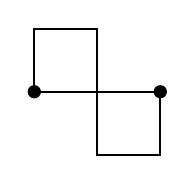
\begin{tikzpicture}[baseline=(current bounding box.center), scale=0.8]
        \bicomplex
        \bicomplexdot{(0,1)}
        \bicomplexdot{(2,1)}
    \end{tikzpicture}
    & 
    $\displaystyle H_{-,0}^{+,0} := \frac{\ker \partial[0,(+,0)]}{\im \partial[(-,0),0]}$
    & 
    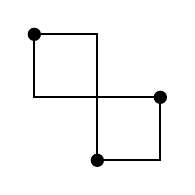
\begin{tikzpicture}[baseline=(current bounding box.center), scale=0.8]
        \bicomplex
        \bicomplexdot{(0,2)}
        \bicomplexdot{(2,1)}
        \bicomplexdot{(1,0)}
    \end{tikzpicture}
    & 
    $\displaystyle H_{-}^{(0,+), (+,0)} := \frac{\ker \partial[0,(+,0)] \cap \ker \partial[0,(0,+)]}{\im \partial[-,0]}$ \\[8ex]
    %%%%%%%%%%%%%%%%%%%%%%%%%%%%%
    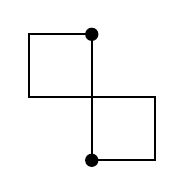
\begin{tikzpicture}[baseline=(current bounding box.center), scale=0.8]
        \bicomplex
        \bicomplexdot{(1,2)}
        \bicomplexdot{(1,0)}
    \end{tikzpicture}
    & 
    $\displaystyle H_{-,0}^{+,0} := \frac{\ker \partial[0,(0,+)]}{\im \partial[(0,-),0]}$
    & 
    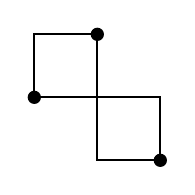
\begin{tikzpicture}[baseline=(current bounding box.center), scale=0.8]
        \bicomplex
        \bicomplexdot{(0,1)}
        \bicomplexdot{(1,2)}
        \bicomplexdot{(2,0)}
    \end{tikzpicture}
    & 
    $\displaystyle H_{(-,0), (0,-)}^{+,-} := \frac{\ker \partial[0,+]}{\im \partial[(-,0),0] + \im \partial[(0,-),0]}$ \\
\end{tabular}
\end{center}

In thre dimensions we have the following commutative diagram:
\begin{center}
    \begin{tikzcd}[row sep=1.5cm, column sep=0.5cm]
                                                & {A(-,-,0)} \arrow[rr] \arrow[dd] &                                  & {A(0,-,0)} \arrow[dd]              &                                  &                                  &                       \\
    {A(-)} \arrow[ru] \arrow[rr] \arrow[dd] &                                  & {A(0,-,-)} \arrow[ru] \arrow[dd] &                                    & {A(0,0,+)} \arrow[rr] \arrow[dd] &                                  & {A(+,0,+)} \arrow[dd] \\
                                                & {A(-,0,0)} \arrow[rr]            &                                  & A \arrow[ru] \arrow[dd] \arrow[rr] &                                  & {A(+,0,0)} \arrow[ru] \arrow[dd] &                       \\
    {A(-,0,-)} \arrow[rr] \arrow[ru]            &                                  & {A(0,0,-)} \arrow[ru]            &                                    & {A(0,+,+)} \arrow[rr]            &                                  & {A(+)}            \\
                                                &                                  &                                  & {A(0,+,0)} \arrow[rr] \arrow[ru]   &                                  & {A(+,+,0)} \arrow[ru]            &                      
    \end{tikzcd}
\end{center}

We have the following \(18\) comological objects:
\begin{center}
    \setlength{\tabcolsep}{7pt} 
    
    \begin{tabular}{ccccc}
        \homologyDiag{1}{ \ldot{-1}{0}{0} }{ \ldot{1}{0}{0} \ldot{0}{0}{1} } &
        \homologyDiag{2}{ \ldot{-1}{-1}{0} }{ \ldot{1}{0}{0} \ldot{0}{1}{0} } &
        \homologyDiag{3}{ \ldot{0}{-1}{-1} }{ \ldot{0}{1}{0} \ldot{0}{0}{1} } &
        \homologyDiag{4}{ \ldot{-1}{-1}{0} \ldot{-1}{0}{-1} }{ \ldot{1}{0}{0} \ldot{0}{1}{1} } &
        \homologyDiag{5}{ \ldot{-1}{-1}{0} \ldot{0}{-1}{-1} }{ \ldot{1}{0}{0} \ldot{0}{1}{1} } \\[1.5cm] % Spazio verticale tra le righe

        \homologyDiag{6}{ \ldot{-1}{0}{-1} \ldot{0}{-1}{-1} }{ \ldot{1}{0}{0} \ldot{0}{1}{1} } &
        \homologyDiag{7}{ \ldot{0}{-1}{-1} \ldot{-1}{0}{0} }{ \ldot{1}{1}{0} \ldot{1}{0}{1} } &
        \homologyDiag{8}{ \ldot{0}{-1}{-1} \ldot{-1}{0}{0} }{ \ldot{1}{1}{0} \ldot{0}{1}{1} } &
        \homologyDiag{9}{ \ldot{0}{-1}{-1} \ldot{-1}{0}{0} }{ \ldot{0}{1}{1} \ldot{1}{0}{1} } &
        \homologyDiag{10}{ \ldot{0}{0}{-1} \ldot{-1}{0}{0} }{ \ldot{1}{0}{1} } \\[1.5cm]

        \homologyDiag{11}{ \ldot{0}{0}{-1} \ldot{0}{-1}{0} }{ \ldot{0}{1}{1} } &
        \homologyDiag{12}{ \ldot{-1}{0}{0} \ldot{0}{-1}{0} }{ \ldot{1}{1}{0} } &
        \homologyDiag{13}{ \ldot{0}{0}{-1} \ldot{-1}{0}{0} \ldot{0}{-1}{0} }{ \ldot{1}{1}{1} } &
        \homologyDiag{14}{ \ldot{-1}{0}{-1} \ldot{0}{-1}{-1} \ldot{-1}{-1}{0} }{ \ldot{1}{1}{0} \ldot{0}{1}{1} \ldot{1}{0}{1} } &
        \homologyDiag{15}{ \ldot{-1}{-1}{-1} }{ \ldot{0}{1}{0} \ldot{1}{0}{0} \ldot{0}{0}{1} } \\

        &
        \homologyDiag{16}{ \ldot{1}{0}{0} }{ \ldot{-1}{0}{0} } &
        \homologyDiag{17}{ \ldot{0}{1}{0} }{ \ldot{0}{-1}{0} } &
        \homologyDiag{18}{ \ldot{0}{0}{1} }{ \ldot{0}{0}{-1} } &
    \end{tabular}
\end{center}

\begin{align*}
    (1) \quad &H_{(-,0,0)}^{(+,0,0), (0,0,+)} := \frac{\ker \partial[0,(+,0,0)] \cap \ker \partial[0,(0,0,+)]}{\im \partial[(-,0,0),0]} \\
    (2) \quad &H_{(-,-,0)}^{(+,0,0), (0,+,0)} := \frac{\ker \partial[0,(+,0,0)] \cap \ker \partial[0,(0,+,0)]}{\im \partial[(-,-,0),0]} \\
    (3) \quad &H_{(0,-,-)}^{(0,+,+), (0,0,+)} := \frac{\ker \partial[0,(0,+,0)] \cap \ker \partial[0,(0,0,+)]}{\im \partial[(0,-,-),0]} \\
    (4) \quad &H_{(-,-,0), (-,0,-)}^{(+,0,0), (0,+,+)} := \frac{\ker \partial[0,(+,0,0)] \cap \ker \partial[0,(0,+,+)]}{\im \partial[(-,-,0),0] + \im \partial[(-,0,-),0]} \\
    (5) \quad &H_{(-,-,0), (0,-,-)}^{(+,0,0), (0,+,+)} := \frac{\ker \partial[0,(+,0,0)] \cap \ker \partial[0,(0,+,+)]}{\im \partial[(-,-,0),0] + \im \partial[(0,-,-),0]} \\
    (6) \quad &H_{(-,0,-), (0,-,-)}^{(+,0,0), (0,+,+)} := \frac{\ker \partial[0,(+,0,0)] \cap \ker \partial[0,(0,+,+)]}{\im \partial[(-,0,-),0] + \im \partial[(0,-,-),0]} \\
    (7) \quad &H_{(0,-,-), (-,0,0)}^{(+,+,0), (+,0,+)} := \frac{\ker \partial[0,(+,+,0)] \cap \ker \partial[0,(+,0,+)]}{\im \partial[(0,-,-),0] + \im \partial[(-,0,0),0]} \\
    (8) \quad &H_{(0,-,-), (-,0,0)}^{(+,+,0), (0,+,+)} := \frac{\ker \partial[0,(+,+,0)] \cap \ker \partial[0,(0,+,+)]}{\im \partial[(0,-,-),0] + \im \partial[(-,0,0),0]} \\
    (9) \quad &H_{(0,-,-), (-,0,0)}^{(0,+,+), (+,0,+)} := \frac{\ker \partial[0,(0,+,+)] \cap \ker \partial[0,(+,0,+)]}{\im \partial[(0,-,-),0] + \im \partial[(-,0,0),0]} \\
    (10) \quad &H_{(0,0,-), (-,0,0)}^{(+,0,+)} := \frac{\ker \partial[0,(+,0,+)]}{\im \partial[(0,0,-),0] + \im \partial[(-,0,0),0]} \\
    (11) \quad &H_{(0,0,-), (0,-,0)}^{(0,+,+)} := \frac{\ker \partial[0,(0,+,+)]}{\im \partial[(0,0,-),0] + \im \partial[(0,-,0),0]} \\
    (12) \quad &H_{(-,0,0), (0,-,0)}^{(+,+,0)} := \frac{\ker \partial[0,(+,+,0)]}{\im \partial[(-,0,0),0] + \im \partial[(0,-,0),0]} \\
    (13) \quad &H_{(0,0,-), (-,0,0), (0,-,0)}^{+} := \frac{\ker \partial[0,+]}{\im \partial[(0,0,-),0] + \im \partial[(-,0,0),0] + \im \partial[(0,-,0),0]} \\
    (14) \quad &H_{(-,0,-), (0,-,-), (-,-,0)}^{(+,+,0), (0,+,+), (+,0,+)} := \frac{\ker\partial[0,(+,+,0)] \cap \ker\partial[0,(0,+,+)] \cap \ker\partial[0,(+,0,+)]}{\im \partial[(-,0,-),0] + \im \partial[(0,-,-),0] + \im \partial[(-,-,0),0]} \\
    (15) \quad &H_{-}^{(0,+,0), (+,0,0), (0,0,+)} := \frac{\ker \partial[0,(0,+,0)] \cap \ker \partial[0,(+,0,0)] \cap \ker \partial[0,(0,0,+)]}{\im \partial[-,0]} \\
    (16) \quad & H_{-,0,0}^{+,0,0} := \frac{
        \ker \partial[0,(+,0,0)]
    }{
        \im \partial[(-,0,0),0]
    } \\
    (17) \quad &H_{0,-,0}^{0,+,0} := \frac{
        \ker \partial[0,(0,+,0)]
    }{
        \im \partial[(0,-,0),0]
    } \\
    (18) \quad &H_{0,0,-}^{0,0,+} := \frac{
        \ker \partial[0,(0,0,+)]
    }{
        \im \partial[(0,0,-),0]
    }
\end{align*}

\pagebreak

\subsection{Generalization of extramural maps}

Cominciamo generalizzando il concetto di \emph{donor} e \emph{receptor}
come i gruppi comologici perfettamente diagonali che traversano l'oggetto centrale.

\begin{definition}
    The \emph{\(n\)-receptor} centered at \(x\) is defined as
    \[
        R(x) := \frac{
            \displaystyle\bigcap_{i=1}^n \ker \partial[x, x + e_i]
        }{
            \im \partial[x-1, x]
        }
        = H_{-1}^{e_1, \cdots, e_n}(x)
    \]
\end{definition}

\begin{definition}
    The \emph{\(n\)-donor} centered at \(x\) is defined as
    \[
        D(x) := \frac{
            \ker \partial[x,x+1]
        }{
            \displaystyle\sum_{i=1}^n \im \partial[x-e_i, x]
        }
        = H_{-e_1, \cdots, -e_n}^1
    \]
\end{definition}

\begin{definition}
    The \emph{\(i\)-axial cohmology} centered at \(x\) is defined as
    \[
        H_i(x) := \frac{
            \ker \partial[x,x+e_i]
        }{
            \im \partial[x-e_i, x]
        }
        = H_{-e_i}^{e_i}
    \]
    for \(i \in \{1, \cdots, n\}\).
\end{definition}

Cominciamo dimostrando esplicitamente il lemma 1.4 del paper originale
per poi generalizzarlo.

\begin{lemma}
    Each arrow \(f \colon A \to B\) in a double complex induces an arrow \(A_\bx \to {}^\bx B\):
\end{lemma}

\begin{proof}
    Without loss of generality, let us consider the horizontal case:
    \begin{center}
        % https://tikzcd.yichuanshen.de/#N4Igdg9gJgpgziAXAbVABwnAlgFyxMJZARgBpiBdUkANwEMAbAVxiRAEEQBfU9TXfIRQAmclVqMWbAELdeIDNjwEiABjHV6zVohAAdPQCMmDBjBxy+SwUQDMGidrYHjp85YX9lQkqVXitKV0XEzMLHisBFRE-AMkdfSNQ9wjPa2jfYTinYKS3cPlFKJ9RLM145zyw7nEYKABzeCJQADMAJwgAWyRREBwIJHUQBjpDGAYABS8bXTMWi3KckDoPdq7B6n6kMkcgkBbVju7EHa3Ee12EqBBqEbHJ6ejhmHnD9cQAFk2BxCHAhMMN2Go3GU3SQhAbSw9QAFgVWkckABWb7bVJrY5fPo-JHoxG-VGIABsePeRMJAHZScdTj8KYs9gBjN6Ywk7BhYMBXOhwGF1IF3UGPCFzBaXNhoFkbbFIenDTnc3n8hkJACONS4QA
        \begin{tikzcd}
                            & \bullet \arrow[d, "b"'] \arrow[r] \arrow[rd, "p", dashed] & \bullet \arrow[d]               &         \\
        \bullet \arrow[r, "a"] & A \arrow[r, "f"] \arrow[d] \arrow[rd, "q", dashed]        & B \arrow[r, "d"] \arrow[d, "c"] & \bullet \\
                            & \bullet \arrow[r]                                         & \bullet                         &        
        \end{tikzcd}
    \end{center}
    \[
        A_\bx = \frac{
            \ker q
        }{
            \im a + \im b
        },
        \quad
        {}^\bx B = \frac{
            \ker c \cap \ker d
        }{
            \im p
        }
    \]
    Let \[
        K := \ker q, \quad M := \im a + \im b, \quad H := \ker c \cap \ker d, \quad N := \im p
    \]
    we need to show that \(f \colon A \to B\) induces a map
    \(K/M \to H/N\).
    We need to ensure that the quotients are well-defined, meaning that \(\im a + \im b \subseteq \ker q\) and \(\im p \subseteq \ker c \cap \ker d\).
    Since the rows and columns are complexes and the squares commute, these inclusions hold.
    \begin{itemize}
        \item \emph{\(f\) sends \(\ker q\) into \(\ker c \cap \ker d\)}:
        let \(\iota_K \colon \ker q \hookrightarrow A\) and \(\iota_H \colon \ker c \cap \ker d \hookrightarrow B\) be the canonical inclusions.
        By definition of \(q\) and \(\ker q\), \(q \iota_K = cf\iota_K = 0\).
        By the properties of the complex, \(df = 0\) and thus \(df\iota_K = 0\).
        Thus, \(f\iota_K \colon K \fromto B\) is nullified both by \(d\) and \(c\).
        By the universal property of the intersection of kernels, meaning the pullback of \(\ker c \cap \ker d\),
        there exists a unique morphism \(\tilde f \colon K \fromto H\) such that
        \(\iota_H \tilde f = f\iota_K\). Thus, \(f\) is restricted to \(\tilde f \colon \ker q \to \ker c \cap \ker d\).
        \item \emph{\(\tilde f\) sends \(\im a + \im b\) into \(\im p\):}
        we can separately check \(\im a\) and \(\im b\).
        By the properties of the complex, \(fa = 0\) meaning that \(fa\) factors through the suboject \(\im p \hookrightarrow B\)
        via the zero morphism.
        By definition of \(p\), \(fb = p\) and thus the image of \(fb\) is contained in \(\im p\).
        By the universal property of the sum of subobjects, \(\im a + \im b\) is the smallest object
        of \(A\) containing both \(\im a\) and \(\im b\).
    \end{itemize}
    We now have the following diagram:
    % https://tikzcd.yichuanshen.de/#N4Igdg9gJgpgziAXAbVABwnAlgFyxMJZABgBpiBdUkANwEMAbAVxiRAFkQBfU9TXfIRRkAjFVqMWbAHLdeIDNjwEiI8uPrNWiEAGk5fJYNWkx1TVJ0AJAwv7KhyAEzrzk7XoD0nHoYEqUFzMJLTYrT1kucRgoAHN4IlAAMwAnCABbJDUQHAgkAGZqHDosBjYACwgIAGtbVIykMhy8xBcckrKdSpq6tMzEJtys3xB6-rahxEKQBjoAIxgGAAV7Yx0UrFjynBA3UJ0AHQO8BlgAAiTehqmiloBWanKYOig2HAB3CCeXhD3LECOaCwAH0bNRZgtlqsAiANlsdiMxkgJi0ACyPZ6vHQfL6Y34zeaLFZGGEMGBJHZ-DyAkH6RF9JDo5pIB4zLBgDxQOhwJ6vKlsI5zOgpC7cChcIA
    \begin{tikzcd}
        M \arrow[r, hook] \arrow[d] & K \arrow[d, "\tilde f"'] \arrow[r, "\pi_K", two heads] & K/M \arrow[d, "\bar f", dashed] \\
        N \arrow[r, hook]           & H \arrow[r, "\pi_H"', two heads]                       & H/N                            
    \end{tikzcd}
    with \(\pi_K \colon K \to K/M\) and \(\pi_H \colon H \to H/N\) canonical projections.

    Since \(\pi_H \tilde f\) vanishes on \(M\), by the universal property of the cokernel of \(M \hookrightarrow K\),
    there exists a unique morphism \(\bar f \colon K/M \to H/N\) such that \(\bar f \pi_K = \pi_H \tilde f\).
    Thus, there exists a unique map
    \[
        \bar f \colon \frac{\ker q}{\im a + \im b} \to \frac{\ker c \cap \ker d}{\im p} 
    \]
    induced by \(f\).
\end{proof}

% Element-wise proof
%Let \([x] \in A_\bx\). Then,
%the induced map \(\tilde f \colon A_\bx \to {}^\bx B\) is given by
%\([x] \mapsto [f(x)]\).
%It suffices to show that this map maps elements from \(\ker q\) into \(\ker c \cap \ker d\)
%and elements from \(\im a + \im b\) into \(\im p\).
%\begin{itemize}
%    \item Let \(x \in \ker q\).
%    Then, \(q(x) = 0 = c(f(x))\) and thus \(f(x) \in \ker c\).
%    By the definition of cochain, \(d(f(x)) = (d\circ f)(x) = 0\)
%    and thus \(f(x) \in \ker d\). We conclude that \(f(x) \in \ker c \cap \ker d\).
%    \item Let \(x \in \im a + \im b\), meaning \(x = a(y) + b(z)\) for some \(y\) and \(z\).
%    We have that \(f(b(z)) = p(z) \in \im p\) by commutativity, and by the
%    definition of cochain \(f(a(y)) = (f \circ a)(y) = 0\).
%    Thus, \(f(x) = f(a(y) + b(z)) = f(a(y)) + f(b(z)) = 0 + p(x) = p(x) \in \im p\).
%\end{itemize}

Written using our notation, this lemma states that for \(n=2\), a morphism \(\partial[x,x+e_i]\) induces
a morphism \(D(x) \to R(x + e_i)\) for every \(i \in \{1, 2\}\).
The same lemma does not generalize for \(n>2\).

\begin{proof}
    Consider the following 
    counterexample: we consider \(\mathbf{Vect}_{\mathbb K}\) for some field \(\mathbb K\).
    We construct a \(3\)-cocomplex where all the objects are zero except for
    \[
        A = \mathbb K, \quad A_{1,0,0} = \mathbb K, \quad A_{1,0,1} = \mathbb K, \quad A_{0,0,1} = \mathbb K = B
    \]
    All the maps are the null maps, except the maps
    between the latter objects which are the identity \(\operatorname{id}_{\mathbb K}\).

    \begin{minipage}{0.5\textwidth}
        % General diagram
        % https://tikzcd.yichuanshen.de/#N4Igdg9gJgpgziAXAbVABwnAlgFyxMJZAJgBoBWAXVJADcBDAGwFcYkQAdDgI2ccZg4QAX1LpMufIRRkAzNTpNW7AIIixIDNjwEiAFlLyaDFm0ScefAUNHjtU-RQUnl5rr36D1dybpSzSYmclMxAAIW9NCR1pZHJA4NN2dysvWyj7PzjSPUTXCw9rSK1fWICABjzQlM8bDRKYojIARirky1ri6IcUctJW4xD2wrT67qzm0krBpLcOovSGnuQ+o0VZgtS6n0aUSaCZ-JqFsczYydzD0K6zxwH1-JvSogDLh+r5tIUYKABzeCIoAAZgAnCAAWyQkxAOAgSD06VBEPhNFhSHIiLBkMQ0LRiGImORONRcMQ5UJ2L6MNJsgpSAC1KQADY6fiSejWWRGYhaRokdj4tyWXysUgAOzsxAIkVEgAckuarIl3NlrIAnAryTLsc0qXixerJartVDcaTFSbEBruc0LcDRTiuXjpfaibqFQTLc0GXi7SB+SibS7-Q7bR7WWbmTRGFgwKEoPQ4AALH4gK7sACOaZAjHo3BgjAACuNpCAQVhfkntiGidbndHY-HEymoNmXKE0Nnc-miyX2OXK9WA2SFRivYK8cLXdiDDaMZRhEA
        \begin{tikzcd}
                                                                            & \bullet \arrow[rr] \arrow[dd] &                                                               & \bullet \arrow[dd] \arrow[ld]      &                               &                    \\
        \bullet \arrow[ru] \arrow[rr] \arrow[dd] \arrow[rrrd, "p"', dashed] &                               & \bullet \arrow[dd]                                            &                                    & {}                            &                    \\
                                                                            & \bullet \arrow[rr]            &                                                               & B \arrow[rr] \arrow[ru] \arrow[dd] &                               & \bullet \arrow[dd] \\
        \bullet \arrow[rr] \arrow[ru]                                       &                               & A \arrow[ru] \arrow[rr] \arrow[dd] \arrow[rrrd, "q"', dashed] &                                    & \bullet \arrow[ru] \arrow[dd] &                    \\
                                                                            & {} \arrow[ru]                 &                                                               & \bullet \arrow[rr]                 &                               & \bullet            \\
                                                                            &                               & \bullet \arrow[rr] \arrow[ru]                                 &                                    & \bullet \arrow[ru]            &                   
        \end{tikzcd}
    \end{minipage}
    \begin{minipage}{0.5\textwidth}
        % Counterexample diagram
        % https://tikzcd.yichuanshen.de/#N4Igdg9gJgpgziAXAbVABwnAlgFyxMJZAJgBoBWAXVJADcBDAGwFcYkQAGEAX1PU1z5CKMgGZqdJq3YAdGQFt6OABYAjVQAIA0jz4gM2PASIAWUuJoMWbRCDmKV67bv6GhpihKvTbXXq8FjFFFSYi8pGzsFJTVNHX99ASNhZHJQ8OtZaMc4l0S3INTSEwyfTjyDQJSQjlLIvz1K5KIyAEY69gaA5pQOUnbLCM6KpPcUVtJawczfEYKUvotJGfKEprHkCbDpsq78qqIJkp3IuYOUMwHlsrOe5BDj6-qeCRgoAHN4IlAAMwAnCDyJATEA4CBIMwgRj0VQwRgABVGQRAfyw72UOBAJyyEDQMD+SggfzA9HkMGAWCg3AA+sB7DEnFpuHl-oCITQwUg0lCYXDEfN2Kj0ZjsbY5Lj8YTiaTyZSaXTsrFtMyEqygYgQZzEGQnji8QSwdKyRSqbT6TllViebCEUjhCAsGBsLAWQD1ZrwYgOKq3Ug+qDPaIfWzECEA0gAGzB9U6rXc7yRcX6qUk41ys2KxnMmjQm3884otEY10h2OB6NcjmeqN6NVIADsVYhFcQAA4mxqW43w22WwBODutb2130a-1a+v9jutlutD3Aqc9uezsvNkchoeD4izsNa1otyF7kyz+ca7fr90diM5x2RKD0ODKN5W3N8u2Cosi3W2ACOJfVA49pCjC3uw96Ps+or6C+vK2gKthCsWLbjp6rTkLO3JajWvyjoeqHoZQ3BAA
        \begin{tikzcd}
                                                                    & 0 \arrow[rr] \arrow[dd] &                                                                                                                                                      & 0 \arrow[dd] \arrow[ld]                                                      &                                                                   &                      \\
        0 \arrow[ru] \arrow[rr] \arrow[dd] \arrow[rrrd, "p"', dashed] &                         & 0 \arrow[dd]                                                                                                                                         &                                                                              & {}                                                                &                      \\
                                                                    & 0 \arrow[rr]            &                                                                                                                                                      & \mathbb K \arrow[rr, "\operatorname{id}_{\mathbb K}"'] \arrow[ru] \arrow[dd] &                                                                   & \mathbb K \arrow[dd] \\
        0 \arrow[rr] \arrow[ru]                                       &                         & \mathbb K \arrow[ru, "\operatorname{id}_{\mathbb K}"'] \arrow[rr, "\operatorname{id}_{\mathbb K}" description] \arrow[dd] \arrow[rrrd, "q"', dashed] &                                                                              & \mathbb K \arrow[ru, "\operatorname{id}_{\mathbb K}"'] \arrow[dd] &                      \\
                                                                    & {} \arrow[ru]           &                                                                                                                                                      & 0 \arrow[rr]                                                                 &                                                                   & 0                    \\
                                                                    &                         & 0 \arrow[rr] \arrow[ru]                                                                                                                              &                                                                              & 0 \arrow[ru]                                                      &                     
        \end{tikzcd}
    \end{minipage}
    The diagram commutes as the compositions of the non-trivial quare are still the identity.
    We will now compute the donor of \(A\), \(D(0)\) and the receiver of \(B\), \(R(e_3)\).
    \begin{enumerate}
        \item \emph{donor of \(A\):} we have \[
            D(0) = \frac{\ker \partial[0,1]}{
                \im \partial[-e_1, 0]
                + \im \partial[-e_2, 0]
                + \im \partial[-e_3, 0]
            }
        \]
        In particular, every monotone path from coordinates \(0\) to \(1\) must go through the second dimension (downwards), which is the zero morphism. Thus,
        \(\partial[0,1] = 0\). This means that every element of \(\mathbb K\) is sent to \(0\) and thus \(\ker\partial[0,1] = \mathbb K\).
        Furthermore, \(A_{-e_1} = A_{-e_2} = A_{-e_3} = 0\) meaning that \[
            \im \partial[-e_1, 0]
            + \im \partial[-e_2, 0]
            + \im \partial[-e_3, 0] = 0
        \]
        Thus, \(D(0) = \mathbb K\).
        \item \emph{receiver of \(B\):} we have \[
            R(e_3) = \frac{
                \ker \partial[e_3,e_3 + e_1]
                \cap \ker \partial[e_3,e_3 + e_2]
                \cap \ker \partial[e_3,2e_3]
            }{
                \im \partial[e_3-1, e_3]
            }
        \]
        For the kernels we have \[
            \ker \partial[e_3,2e_3]
            \cap \ker \partial[e_3,e_3 + e_2]
            \cap \ker \partial[e_3,e_3 + e_1]
            = \ker 0 \intersection \ker 0 \intersection \ker \operatorname{id}_{\mathbb K} = 0
        \]
        Furtermore, \(A_{e_3 - 1} = A_{-1, -1, 0} = 0\), and thus \(\im p = 0\).
        Thus, \(R(e_3)=0\).
    \end{enumerate}
    Suppose that \(f = \operatorname{id}_{\mathbb K} \colon A \to B\) 
    induces a morphism \(D(0) \to R(e_3)\).
    Then, \(f\) must send elements of the numerator of \(D(0)\) into the numerator of \(R(e_3)\), meaning
    \[
        f(\ker \partial[0,1]) \subseteq \ker \partial[e_3,e_3 + e_1]
        \cap \ker \partial[e_3,e_3 + e_2]
        \cap \ker \partial[e_3,2e_3]
    \]
    However, \(\ker \partial[0,1] = \mathbb K\)
    and \(f = \operatorname{id}_{\mathbb K} \colon A_0 \to A_{e_3}\)
    meaning that \(f\) doe snot factor through the zero subobject \(0 \hookrightarrow A_{e_3}\).
    In particular the arrow \(f \colon A_0 \to A_{e_3}\) does not restrict to an arrow
    \[
        \ker \partial[0,1] \to \ker \partial[e_3,e_3 + e_1]
        \cap \ker \partial[e_3,e_3 + e_2]
        \cap \ker \partial[e_3,2e_3]
    \]
    Thus, \(f\) does not induce such a map.
\end{proof}

Se provassimo a dimostrare il lemma falso per \(n=3\),
l'unica inclusione che funziona sempre, sia per i nuclei che per le immagini,
è quella nella direzione del morfismo iniziale.
Considerando la definizione delle mappe diagonali, possiamo solamente
dire l'ultima delle tre mappe composte viene
annullata dal nucleo della mappa diagonale, ma ci servirebbe
che pure le doppie composizioni vengano annullate, cioè ci servirebbe
che l'oggetto comologico avesse intersezioni di nuclei di composizioni di due mappe,
non solo una. Lo stesso ragionamento vale per il denominatore con le immagini.
Notiamo che un tale oggetto è precisamente l'oggetto numerato (14),
che è una sorta di middle object, sia donor che receiver.
Allora, l'oggetto (13) mappa naturalmente nell'oggetto (14), non
il (15) come dimostratosi, mentre l'oggetto (14) mappa naturalmente
nell'oggetto (15). Possiamo quindi estendere il lemma originale aggiungendo un passaggio intermedio.

Abbiamo allora il seguente lemma.

\begin{lemma}
    Each pair of arrows in a triple complex
    \begin{center}
        % https://tikzcd.yichuanshen.de/#N4Igdg9gJgpgziAXAbVABwnAlgFyxMJZABgBpiBdUkANwEMAbAVxiRAEEQBfU9TXfIRQBGclVqMWbAELdeIDNjwEiAJjHV6zVohABhbuJhQA5vCKgAZgCcIAWyRkQOCElETtbS3Ku2HidxckdRAGOgAjGAYABX5lIVCYSxwQTUkdEBNDLiA
        \begin{tikzcd}
        A_x \arrow[r, "f"] & A_{x+e_i} \arrow[r, "g"] & A_{x+e_i+d_j}
        \end{tikzcd}
    \end{center}
    for every \(i,j \in \{1, \cdots, n\}\) with \(i \neq j\),
    induces the arrows
    \begin{center}
        % https://tikzcd.yichuanshen.de/#N4Igdg9gJgpgziAXAbVABwnAlgFyxMJZABgBpiBdUkANwEMAbAVxiRABEAKAQQEoQAvqXSZc+QigCM5KrUYs2AWU4AhfkJHY8BIgCYZ1es1aIQAJU4BhdbJhQA5vCKgAZgCcIAWyRkQOCEiSGiDuXoHU-kj6IAx0AEYwDAAKotoSMTAuOIIUAkA
        \begin{tikzcd}
        D(A_x) \arrow[r] & M(A_{x+e_i}) \arrow[r] & R(A_{x+e_i + e_j})
        \end{tikzcd}
    \end{center}
    where \[
        M(x) := \frac{
            \ker \partial[x, x + e_1 + e_2]
            \intersection
            \ker \partial[x, x + e_2 + e_3]
            \intersection
            \ker \partial[x, x + e_1 + e_3]
        }{
            \im \partial[x - e_1 - e_2, x]
            +
            \im \partial[x - e_2 - e_3, x]
            +
            \im \partial[x - e_1 - e_3, x]
        }
        = H_{(-,0,-), (0,-,-), (-,-,0)}^{(+,+,0), (0,+,+), (+,0,+)}(x)
    \]
\end{lemma}

Questo lemma può essere ulteriore generalizzato a \(n\)-complessi.
Se consideriamo il lemma generalizzato per \(n=3\), notiamo che il
donatore è costruito considerando kernel di mappe di lunghezza \(3\) (composizione di \(3\) morfismo),
di cui ce n'è uno solo, e immagini di mappe di lunghezza \(1\), ci cui ce ne sono \(3\).
L'oggetto intermedio è costruito con kernel e immagini di mappe entrambe di lunghezza 3.
Infine, il receiver è costituito da nuclei di mappe di lunghezza uno e immagini di mappe di lunghezza \(3\).
Per ognuno di questi tre oggetti, consideriamo le tuple \((a,b)\) dove \(a\) è la lunghezza
dei morfismi di cui vengono considerate le immagini e \(b\) è la lunghezza dei morfismi di cui vengono considerati i kernel.
Il lemma ci dà quindi una successione di mappe della forma \((1,3) \to (2,2) \to (3,1)\).
Questa simmetria ci suggerisce che il lemma possa essere generalizzato da un \(n\) complessi
con una successione di mappe fra \(n\) oggetti comologici diagonali della forma
\[
    (1,n) \to (2, n-1) \to \cdots \to (n-1, 2) \to (n,1)
\]
Definiamo quindi oggetti comologici diagonali che seguono questa forma.

\begin{definition}
    Sia \(1 \leq k \leq n\). Definiamo il \emph{\(k\)-diagonal cohomological object} as
    \[
        M_k(x) := \frac{
            \displaystyle
            \bigcap_{
                \substack{
                    J \subseteq \{1, \cdots, n\} \\
                    |J| = n-k+1
                }
            } \ker\partial\left[
                x, x + e_J
            \right]
        }{
            \displaystyle
            \sum_{
                \substack{
                    J \subseteq \{1, \cdots, n\} \\
                    |J| = k
                }
            } \im\partial\left[
                x - e_J, x
            \right]
        }
    \]
\end{definition}

\begin{proposition}
    L'oggetto \(M_k(x)\) è ben definito.
    % TODO Mostrare che questi sono effettivamente oggetti della forma di Bergman?
\end{proposition}

\begin{proof}
    Siano \(K_k(x) = \bigcap \ker \partial[x,x+e_J]\) e
    \(I_k(x) = \sum \im \partial[x-e_J, x]\) cosicché \(M_k(x) = K_k(x)/I_k(x)\).
    Bisogna mostrare che \(I_k(x) \subseteq K_k(x)\).
    Fissiamo \(S,T \subseteq \{1, \cdots, n\}\) tali che
    \(|S| = n-k+1\) e \(|T| = k\).
    Naturalmente, \(|S| + |T| = n+1 > n\) e quindi \(S \cap T \neq \varnothing\).
    Sia \(i \in S \cap T\) e consideriamo il composto
    \begin{center}
        % https://tikzcd.yichuanshen.de/#N4Igdg9gJgpgziAXAbVABwnAlgFyxMJZABgBpiBdUkANwEMAbAVxiRAEEB9YADwFoYnACoBfECNLpMufIRQBGclVqMWbLj3GSQGbHgJEATEur1mrRB248A1IIDKYkcphQA5vCKgAZgCcIALZIZCA4EEiKKuZsADoxaHS+eIzI-IJCpDwUWj7+QYiRYUjGUWqWcQlJWCk8mXac9tkSuYHB1EWIJQBGMGBQSHwAzCFmZSAVickMqQLCdQ7Z1Ax0PQwACtL6ciC+WG4AFjjiFCJAA
        \begin{tikzcd}
        A_{x-e_T} \arrow[r, "{\partial[x-e_T,x]}"] \arrow[rr, "{\partial[x-e_T,x+e_S]}"', bend right] & A_x \arrow[r, "{\partial[x,x+e_S]}"] & A_{x+e_S}
        \end{tikzcd}
    \end{center}
    In particolare, abbiamo \(e_i \in \#\partial[x-e_T,x] \cap \#\partial[x,x+e_S]\),
    e quindi la direzione \(e_i\) viene traversata \(\geq 2\) volte e quindi per il lemma % TODO: citare
    vale \(\partial[x-e_T, x+e_S] = 0\).
    Dunque, \(\im \partial[x-e_T, x] \subseteq \ker \partial[x, x+e_S]\).
    Per arbitrarietà di \(S\) e \(T\) troviamo che \(I_k(x) \subseteq K_k(x)\).
\end{proof}

Questa è infatti una generalizzazione del donor e del receiver, con quest'ultimi
che si trovano ai rispettivi capi della successione di oggetti.
Infatti, per \(k=1\) ritroviamo il donor
\[
    M_1(x) = \frac{
        \displaystyle
        \bigcap_{
            \substack{
                J \subseteq \{1, \cdots, n\} \\
                |J| = n
            }
        } \ker\partial\left[
            x, x + e_J
        \right]
    }{
        \displaystyle
        \sum_{
            \substack{
                J \subseteq \{1, \cdots, n\} \\
                |J| = 1
            }
        } \im\partial\left[
            x - e_J, x
        \right]
    }
    = \frac{
        \ker\partial\left[
            x, x + \displaystyle\sum_{j=1}^n e_j
        \right]
    }{
        \displaystyle
        \sum_{j=1}^n
        \im\partial\left[
            x - e_j, x
        \right]
    }
    = \frac{
        \ker\partial\left[
            x, x + 1
        \right]
    }{
        \displaystyle
        \sum_{j=1}^n
        \im\partial\left[
            x - e_j, x
        \right]
    } = D(x)
\]
mentre per \(k=n\) ritroviamo il receiver
\[
    M_k(x) = \frac{
        \displaystyle
        \bigcap_{
            \substack{
                J \subseteq \{1, \cdots, n\} \\
                |J| = 1
            }
        } \ker\partial\left[
            x, x + e_J
        \right]
    }{
        \displaystyle
        \sum_{
            \substack{
                J \subseteq \{1, \cdots, n\} \\
                |J| = n
            }
        } \im\partial\left[
            x - e_J, x
        \right]
    }
    = \frac{
        \displaystyle
        \bigcap_{j=1}^n \ker \partial[x, x + e_j]
    }{
        \im \partial\left[
            x - \displaystyle\sum_{j=1}^n e_j, x
        \right]
    }
    = \frac{
        \displaystyle
        \bigcap_{j=1}^n \ker \partial[x, x + e_j]
    }{
        \im \partial\left[
            x - 1, x
        \right]
    } = R(x)
\]
Abbiamo quindi un cammino discreto di oggetti comologici diagonali fra \(D(x)\) e \(R(x)\).

\begin{lemma}
    For every \(x\in\mathbb Z^n\) and every \(i\in\{1,\dots,n\}\), the morphism
    \[
        A_x\to A_{x+e_i}
    \]
    induces a canonical morphism
    \[
        \delta^k_i \colon
        M_k(x)\to M_{k+1}(x+e_i).
    \]
    In particular, let \(i_1, i_2, \cdots, i_{n-1} \in \{1, \cdots, n\}\).
    Then, for every \(x\in\mathbb Z^n\), every sequence of morphisms
    \[
        A_{x} \to
        A_{x + e_{i_1}} \to
        A_{x + e_{i_1} + e_{i_2}} \to
        \cdots \to
        A_{x + \sum_{j=1}^{n-1} e_{i_{j}}}
    \]
    induces a chain of morphisms
    \[
        M_1\left(x\right) \to
        M_2\left(x + e_{i_1}\right) \to
        M_3\left(x + e_{i_1} + e_{i_2}\right) \to
        \cdots \to
        M_{n}\left(x + \sum_{j=1}^{n-1} e_{i,j}\right)
    \]
\end{lemma}

If the indices \(i_1,\dots,i_{n-1}\) are pairwise distinct,
these chains are precisely the maximal paths in the Boolean diagram indexed by subsets of \(\{1,\cdots, n\}\),
meaning that we can construct a Boolean lattice of induced morphism.
In general, we can consider the chains where the indices are not disjoint. However,
by the commutativity of the diagram, we can write such a chain as a path of morphism
such that at least two morphisms in the same direction are adjacent, meaning that the map is null
by the properties of a complex. These kind of map are outside of the Boolean lattice.

We can also count the amount of maximal chains. We need to choose \(n-1\) distict
directions, meaning that the amount of maximal chains is \(n\cdot (n-1)! = n!\).
However, by the commutativity of the diagram, the \((n-1)!\) terminating
in the same vertex are all equa. Thus, there are \(n\) composite maps from the
donor and the receiver.

\begin{proof}
    Fissiamo \(r\) tale che \(1 \leq r < n\) e consideriamo il morfismo \(f \colon A \to B\)
    con \[
        A = A_{x + \sum_{j=1}^{r-1} e_{i_j}}, \quad
        B = A_{x + \sum_{j=1}^{r} e_{i_j}}
    \]
    che ha direzione \(\#f = \{e_{i_r}\}\),
    e mostriamo che questo morfismo induce un morfismo \(M_r(A) \to M_{r+1}(B)\).
    Scriviamo esplicitamente \(M_r(A)\) e \(M_{r+1}(B)\) e introduciamo un cambio di variabile
    per lavorare su uno spazio centrato in \(A\). Abbiamo per \(A\)
    \begin{DispWithArrows*}
        M_r(A) &= \frac{
            \displaystyle\bigcap_{\substack{J \subseteq \{1, \cdots, n\} \\ |J| = n-r+1}}
            \ker\partial\left[
                x + \displaystyle\sum_{j=1}^{r-1} e_{i_j},
                x + \displaystyle\sum_{j=1}^{r-1} e_{i_j} + e_J
            \right]
        }{
            \displaystyle\sum_{\substack{J \subseteq \{1, \cdots, n\} \\ |J| = r}}
            \im\partial\left[
                x + \displaystyle\sum_{j=1}^{r-1} e_{i_j} - e_J,
                x + \displaystyle\sum_{j=1}^{r-1} e_{i_j}
            \right]
        } \Arrow{\(y = \displaystyle\sum_{j=1}^{r-1} e_{i_j}\)} \\
        &= \frac{
            \displaystyle\bigcap_{\substack{J \subseteq \{1, \cdots, n\} \\ |J| = n-r+1}}
            \ker\overbrace{
                \partial\left[
                    y,
                    y + e_J
                \right]
            }^{\partial_{J,n-r+1}}
        }{
            \displaystyle\sum_{\substack{J \subseteq \{1, \cdots, n\} \\ |J| = r}}
            \im\underbrace{
                \partial\left[
                    y - e_J,
                    y
                \right]
            }_{\partial^{J, r}}
        }
    \end{DispWithArrows*}
    Mentre per \(B\) abbiamo
    \begin{DispWithArrows*}
        M_{r+1}(B) &= \frac{
            \displaystyle\bigcap_{\substack{J \subseteq \{1, \cdots, n\} \\ |J| = n-r}}
            \ker\partial\left[
                x + \displaystyle\sum_{j=1}^{r-1} e_{i_j},
                x + \displaystyle\sum_{j=1}^{r-1} e_{i_j} + e_J
            \right]
        }{
            \displaystyle\sum_{\substack{J \subseteq \{1, \cdots, n\} \\ |J| = r+1}}
            \im\partial\left[
                x + \displaystyle\sum_{j=1}^{r} e_{i_j} - e_J,
                x + \displaystyle\sum_{j=1}^{r} e_{i_j}
            \right]
        } \Arrow{\(y = \displaystyle\sum_{j=1}^{r-1} e_{i_j}\)} \\
        &= \frac{
            \displaystyle\bigcap_{\substack{J \subseteq \{1, \cdots, n\} \\ |J| = n-r}}
            \ker\overbrace{
                \partial\left[
                    y + e_{i_r},
                    y + e_{i_r} + e_J
                \right]
            }^{\partial_{J,n-r}}
        }{
            \displaystyle\sum_{\substack{J \subseteq \{1, \cdots, n\} \\ |J| = r+1}}
            \im\underbrace{
                \partial\left[
                    y + e_{i_r} - e_J,
                    y + e_{i_r}
                \right]
            }_{\partial^{J, r+1}}
        }
    \end{DispWithArrows*}
    Siano \(K_k(x) = \bigcap \ker \partial[x,x+e_J]\) e
    \(I_k(x) = \sum \im \partial[x-e_J, x]\) cosicché \(M_k(x) = K_k(x)/I_k(x)\).
    Mostriamo quindi separamente che la mappa manda
    \(K_r(y)\) into \(K_{r+1}(y+e_{i_r})\)
    and \(I_r(y)\) into \(I_{r+1}(y + e_{i_r})\).
    \begin{itemize}
        \item \(f\) manda \(K_r(y)\) in \(K_{r+1}(y + e_{i_r})\): consideriamo un morfismo \(\partial_{J, n-r}\)
        arbitrario della definizione di \(K_{r+1}(y + e_{i_r})\) e mostriamo che esiste sempre
        un morfismo della definizione di \(K_r(y)\) tale per cui \(f\) si restringe
        fra questi due.
        Per costruzione, \(\#f = \{e_{i_r}\}\) che ha lunghezza \(1\) e \(\#\partial_{J, n-r} = \{e_j\}_{j \in J}\)
        con lunghezza \(n-r\) per costruzione di \(J\).
        Consideriamo il morfismo \(\partial_{J,n-r} \circ f\), che connette \(A\) al morfismo
        scelto dalla definizione di \(K_{r+1}(y + e_{i_r})\), e distinguiamo due casi:
        \begin{itemize}
            \item se \(e_{i_r} \in \#\partial_{J,n-r}\), allora \((\partial_{J,n-r} \circ f)\) traversa
            due volte la direzione \(e_{i_r}\). Per il lemma % todo cite
            vediamo immediatamente che vale \(\partial_{J,n-r} \circ f = 0\) sempre.
            \item se \(e_{i_r} \notin \#\partial_{J,n-r}\), allora \((\partial_{J,n-r} \circ f)\) traversa
            solo una volta la direzione \(e_{i_r}\).
            Nella definizione di \(K_{r}(y)\) vengono usati tutti i morfismi partenti da \(A\) di lunghezza
            \(n-r+1\). Fra questi, consideriamo solo quelli che includono un morfismo che traversa la direzione
            \(e_{i_r}\), cioè \[
                E = \left\{
                    \partial_{J, n-r+1} \mid J \subseteq \{1, \cdots, n\} \land |J| = n-r+1 \land i_r \in J
                \right\}
            \]
            Per ogni \(\partial \in E\), possiamo rappresentare \(\partial\) come
            \(\partial = \alpha_1 \circ \cdots \circ \alpha_{n-r+1}\) dove \(|\#\alpha_i| = 1\),
            cioè come composizione di morfismi di lunghezza uno. Per commutatività del diagramma,
            possiamo scegliere tale rappresentazione tale che \(\#\alpha_{n-r+1} = \{e_{i_r}\}\).
            Ma quindi, data una tale rappresentazione, deve essere per forza \(\alpha_{n-r+1} = f\) e possiamo scrivere
            \(\partial = (\alpha_1 \circ \cdots \circ \alpha_{n-r}) \circ f\).
            Per definizione, \(E\) contiene tutti i possibili morfismi di lunghezza \(n-r+1\).
            In particolare, il termine \((\alpha_1 \circ \cdots \circ \alpha_{n-r})\) può assumere
            qualsiasi cammino di lunghezza \(n-r\) che parte da \(fA = B\), e quindi deve esistere
            \(\partial \in E\) tale che \(\partial = \partial_{J,n-r} \circ f\).
            Se consideriamo ora l'inclusione canonica \(\iota \colon \ker \partial \to A\), troviamo che
            \(\partial \iota = \partial_{J,n-r} f \iota = 0\).
            Dunque, per la proprietà universale dell'intersezione dei nuclei, il morfismo
            \[
                \restr{f}{K_r(y)} \colon K_r(y) \to A_{y + e_{i_r}}
            \]
            fattorizza in modo unico attraverso \(K_{r+1}(y + e_{i_r})\) mediante il morfismo
            \[
                \tilde f \colon K_r(y) \to K_{r+1}(y + e_{i_r})
            \]
        \end{itemize}
        \item \(\tilde f\) manda \(I_r(y)\) in \(I_{r+1}(y+e_{i_r})\): Omessa per ora ma stessa forma.
    \end{itemize}
    Per la proprietà universale del quoziente in una categoria abeliana,
    \(\tilde f\) induce un unico morfismo
    \[
        \delta_i^r(y) \colon K_r(y) / I_r(y)
        \to
        K_{r+1}(y + e_{i_r}) / I_{r+1}(y + e_{i_r})
    \]
    cioè \[
        \delta_i^r(x) \colon
        M_r\left(x + \sum_{j=1}^{r-1} e_{i_j}\right)
        \to
        M_{r+1}\left(x + \sum_{j=1}^{r} e_{i_j}\right)
    \]
\end{proof}

\begin{lemma}
    Sia \(S \subseteq \{1, \cdots, n\}\)
    con \(|S| = k-1\) e due direzioni \(i,j \notin S\) con \(i\neq j\).
    Allora, il diagramma indotto
    \begin{center}
        \begin{tikzcd} M_k(x+e_S) \arrow[r, "\delta_i"] \arrow[d, "\delta_j"'] & M_{k+1}(x+e_S+e_i) \arrow[d, "\delta_j"] \\ M_{k+1}(x+e_S+e_j) \arrow[r, "\delta_i"'] & M_{k+2}(x+e_S+e_i+e_j) \end{tikzcd}
    \end{center}
    è un diagramma commutativo.
\end{lemma}

\begin{proof}
    Le due composizioni sono rispettivamente indotte da
    \(\partial_{x + e_S + e_i}^{(j)} \circ \partial_{x + e_S}^{(i)}\)
    e \(\partial_{x + e_S + e_j}^{(i)} \circ \partial_{x + e_S}^{(j)}\).
    Questi due morfismi coincidono per la commutatività dei quadrati dell'\(n\)-cocomplesso.
    Per unicità delle mappe indotte, anche le mappe fra gli oggetti \(M_k\) coincidono.
\end{proof}

\subsection{Generalization of intramural maps}

In generale le mappe vanno dal receiver verso il donor, al contrario delle extramural maps.

Nel caso tridimensionale abbiamo
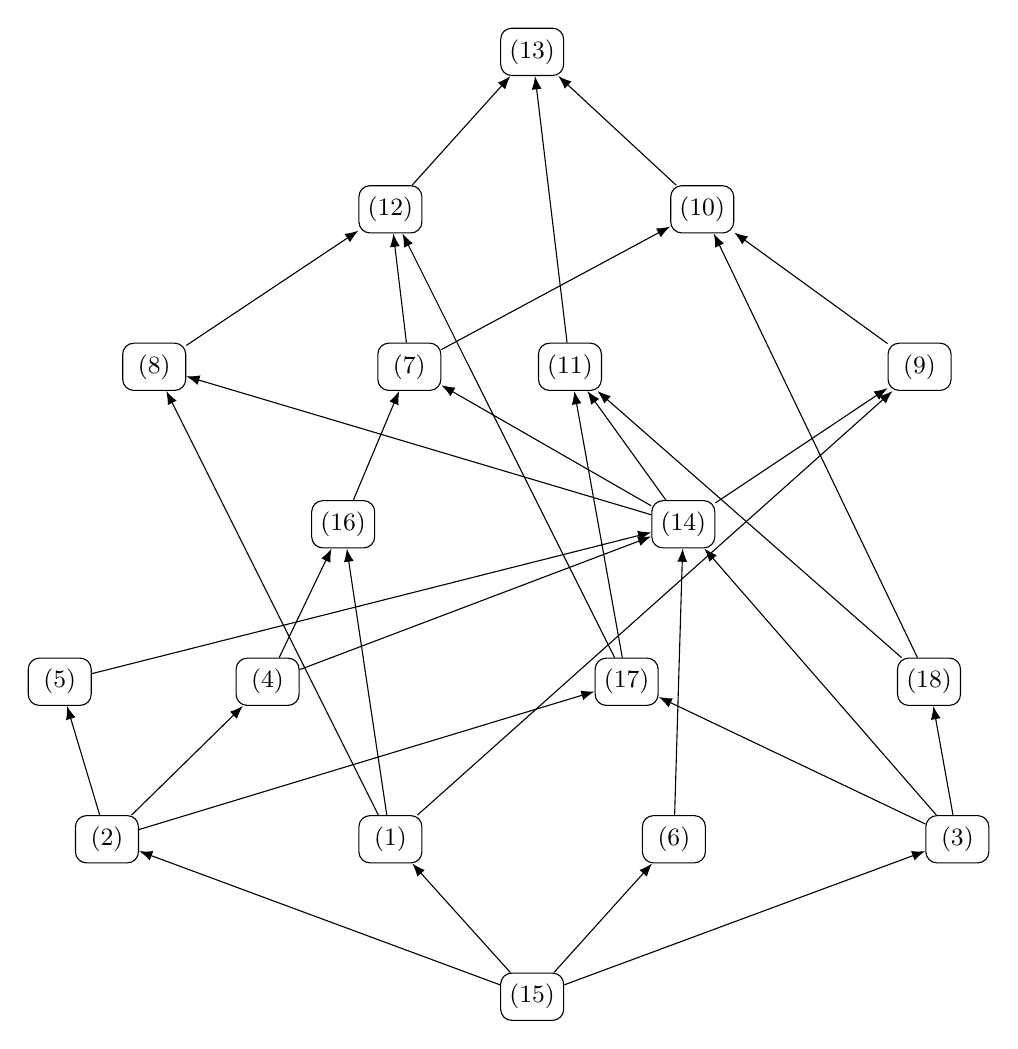
\begin{tikzpicture}[
    >=Latex,
    x=1.2cm, y=1.0cm,
    every node/.style={
        draw,
        rounded corners,
        minimum width=8mm,
        minimum height=6mm,
        inner sep=2pt,
        font=\small
    }
]

%---------------------------------
% Nodes
%---------------------------------

% Level 0
\node (n15) at (0,0) {(15)};

% Level 1
\node (n2)  at (-4.5,2) {(2)};
\node (n1)  at (-1.5,2) {(1)};
\node (n6)  at ( 1.5,2) {(6)};
\node (n3)  at ( 4.5,2) {(3)};

% Level 2
\node (n5)  at (-5.0,4) {(5)};
\node (n4)  at (-2.8,4) {(4)};
\node (n17) at ( 1.0,4) {(17)};
\node (n18) at ( 4.2,4) {(18)};

% Level 3
\node (n16) at (-2.0,6) {(16)};
\node (n14) at ( 1.6,6) {(14)};

% Level 4
\node (n8)  at (-4.0,8) {(8)};
\node (n7)  at (-1.3,8) {(7)};
\node (n11) at ( 0.4,8) {(11)};
\node (n9)  at ( 4.1,8) {(9)};

% Level 5
\node (n12) at (-1.5,10) {(12)};
\node (n10) at ( 1.8,10) {(10)};

% Level 6
\node (n13) at (0,12) {(13)};

%---------------------------------
% Arrows: cover relations only
%---------------------------------

% From (15)
\draw[->] (n15) -- (n1);
\draw[->] (n15) -- (n2);
\draw[->] (n15) -- (n3);
\draw[->] (n15) -- (n6);

% From (1)
\draw[->] (n1) -- (n8);
\draw[->] (n1) -- (n9);
\draw[->] (n1) -- (n16);

% From (2)
\draw[->] (n2) -- (n4);
\draw[->] (n2) -- (n5);
\draw[->] (n2) -- (n17);

% From (3)
\draw[->] (n3) -- (n14);
\draw[->] (n3) -- (n17);
\draw[->] (n3) -- (n18);

% From (6)
\draw[->] (n6) -- (n14);

% From (4)
\draw[->] (n4) -- (n14);
\draw[->] (n4) -- (n16);

% From (5)
\draw[->] (n5) -- (n14);

% From (16)
\draw[->] (n16) -- (n7);

% From (17)
\draw[->] (n17) -- (n11);
\draw[->] (n17) -- (n12);

% From (18)
\draw[->] (n18) -- (n10);
\draw[->] (n18) -- (n11);

% From (14)
\draw[->] (n14) -- (n7);
\draw[->] (n14) -- (n8);
\draw[->] (n14) -- (n9);
\draw[->] (n14) -- (n11);

% From (7)
\draw[->] (n7) -- (n10);
\draw[->] (n7) -- (n12);

% From (8)
\draw[->] (n8) -- (n12);

% From (9)
\draw[->] (n9) -- (n10);

% To the top (13)
\draw[->] (n10) -- (n13);
\draw[->] (n11) -- (n13);
\draw[->] (n12) -- (n13);

\end{tikzpicture}

\pagebreak

\section{Work in progress}

Caso verticale del diagramma del bicomplesso.

\[
\begin{tikzcd}[column sep=3.2em,row sep=3.0em]
{} & U \arrow[d,"c"'] & {} \\
L \arrow[r,"d"'] \arrow[d,"b"'] & A \arrow[r,"e"] \arrow[d,"v"'] & C \arrow[d,"g"] \\
M \arrow[r,"k"'] & B \arrow[r,"h"'] \arrow[d,"m"'] & D \\
{} & N & {}
\end{tikzcd}
\]

\[
D(A)=\frac{\ker(h\circ v)}{\operatorname{im}c+\operatorname{im}d}
      =\frac{\ker(g\circ e)}{\operatorname{im}c+\operatorname{im}d},
\qquad
R(B)=\frac{\ker h\cap\ker m}{\operatorname{im}(v\circ d)}
      =\frac{\ker h\cap\ker m}{\operatorname{im}(k\circ b)}.
\]

Ci piacerebbe dire che un morfismo A->B induce un morfiso D(A) -> D(B)
questo già non è vero per n=3. Controesempio sugli spazi vettoriali.
Che cosa ci servirebbe? Ci servirebbe un donor che ha l'intersezione dei 3 kernel a due step.
Ma questo è l'elemento 14, infatti dati A->B->C abbiamo due mappe indotte D(A) -> M(B) -> R(C).
Abbiamo quindi 3 * 2 = 6 casi, ma per la commutatività metà coincidono quindi 3.


La prima parte di "Generalization of extramural maps" è in realtà
una generalizzazione dei cocomplessi su n-complessi. Spiegare quali sono gli oggetti di Bergman generalizzati
e perché coincidono con il numero di Dedekind.


\end{document}